\chapter{Einleitung}

\section{Aufgabe}
Es ist eine Applikation zu entwickeln welches Gesichter mit mit einem Neuronalen  Netz erkennt. Die gefundenen Gesichter sollen ausgeschnitten werden und in einem Ordner zur Weiterverarbeitung gespeichert werden.

\section{Einführung in die Gesichtserkennung}
Bei der Gesichtserkennung unterscheidet man zwischen Lokalisation von Gesichtern  und der Zuordnung der Gesichter zu einer bestimmten Person.\\%Quelle Wikipedia eintragen. https://de.wikipedia.org/wiki/Gesichtserkennung
\begin{figure}
	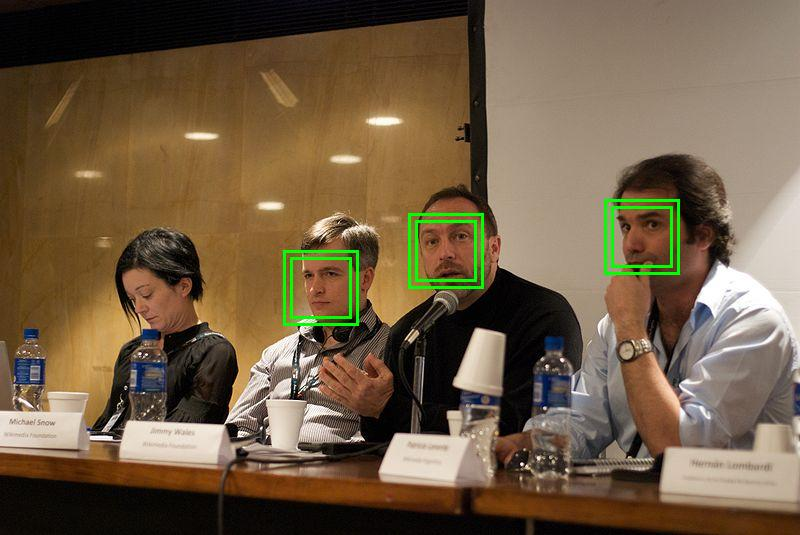
\includegraphics[width=1.0\textwidth]{bilder/face-detection.jpg}	
	\caption{Automatische Gesichtserkennung mit OpenCV.}
\end{figure}
\footnote{\url{https://de.wikipedia.org/wiki/Gesichtserkennung\#/media/File:Face\_detection.jpg}}


